% Options for packages loaded elsewhere
\PassOptionsToPackage{unicode}{hyperref}
\PassOptionsToPackage{hyphens}{url}
%
\documentclass[
]{article}
\usepackage{amsmath,amssymb}
\usepackage{lmodern}
\usepackage{iftex}
\ifPDFTeX
  \usepackage[T1]{fontenc}
  \usepackage[utf8]{inputenc}
  \usepackage{textcomp} % provide euro and other symbols
\else % if luatex or xetex
  \usepackage{unicode-math}
  \defaultfontfeatures{Scale=MatchLowercase}
  \defaultfontfeatures[\rmfamily]{Ligatures=TeX,Scale=1}
\fi
% Use upquote if available, for straight quotes in verbatim environments
\IfFileExists{upquote.sty}{\usepackage{upquote}}{}
\IfFileExists{microtype.sty}{% use microtype if available
  \usepackage[]{microtype}
  \UseMicrotypeSet[protrusion]{basicmath} % disable protrusion for tt fonts
}{}
\makeatletter
\@ifundefined{KOMAClassName}{% if non-KOMA class
  \IfFileExists{parskip.sty}{%
    \usepackage{parskip}
  }{% else
    \setlength{\parindent}{0pt}
    \setlength{\parskip}{6pt plus 2pt minus 1pt}}
}{% if KOMA class
  \KOMAoptions{parskip=half}}
\makeatother
\usepackage{xcolor}
\usepackage[margin=1in]{geometry}
\usepackage{color}
\usepackage{fancyvrb}
\newcommand{\VerbBar}{|}
\newcommand{\VERB}{\Verb[commandchars=\\\{\}]}
\DefineVerbatimEnvironment{Highlighting}{Verbatim}{commandchars=\\\{\}}
% Add ',fontsize=\small' for more characters per line
\usepackage{framed}
\definecolor{shadecolor}{RGB}{248,248,248}
\newenvironment{Shaded}{\begin{snugshade}}{\end{snugshade}}
\newcommand{\AlertTok}[1]{\textcolor[rgb]{0.94,0.16,0.16}{#1}}
\newcommand{\AnnotationTok}[1]{\textcolor[rgb]{0.56,0.35,0.01}{\textbf{\textit{#1}}}}
\newcommand{\AttributeTok}[1]{\textcolor[rgb]{0.77,0.63,0.00}{#1}}
\newcommand{\BaseNTok}[1]{\textcolor[rgb]{0.00,0.00,0.81}{#1}}
\newcommand{\BuiltInTok}[1]{#1}
\newcommand{\CharTok}[1]{\textcolor[rgb]{0.31,0.60,0.02}{#1}}
\newcommand{\CommentTok}[1]{\textcolor[rgb]{0.56,0.35,0.01}{\textit{#1}}}
\newcommand{\CommentVarTok}[1]{\textcolor[rgb]{0.56,0.35,0.01}{\textbf{\textit{#1}}}}
\newcommand{\ConstantTok}[1]{\textcolor[rgb]{0.00,0.00,0.00}{#1}}
\newcommand{\ControlFlowTok}[1]{\textcolor[rgb]{0.13,0.29,0.53}{\textbf{#1}}}
\newcommand{\DataTypeTok}[1]{\textcolor[rgb]{0.13,0.29,0.53}{#1}}
\newcommand{\DecValTok}[1]{\textcolor[rgb]{0.00,0.00,0.81}{#1}}
\newcommand{\DocumentationTok}[1]{\textcolor[rgb]{0.56,0.35,0.01}{\textbf{\textit{#1}}}}
\newcommand{\ErrorTok}[1]{\textcolor[rgb]{0.64,0.00,0.00}{\textbf{#1}}}
\newcommand{\ExtensionTok}[1]{#1}
\newcommand{\FloatTok}[1]{\textcolor[rgb]{0.00,0.00,0.81}{#1}}
\newcommand{\FunctionTok}[1]{\textcolor[rgb]{0.00,0.00,0.00}{#1}}
\newcommand{\ImportTok}[1]{#1}
\newcommand{\InformationTok}[1]{\textcolor[rgb]{0.56,0.35,0.01}{\textbf{\textit{#1}}}}
\newcommand{\KeywordTok}[1]{\textcolor[rgb]{0.13,0.29,0.53}{\textbf{#1}}}
\newcommand{\NormalTok}[1]{#1}
\newcommand{\OperatorTok}[1]{\textcolor[rgb]{0.81,0.36,0.00}{\textbf{#1}}}
\newcommand{\OtherTok}[1]{\textcolor[rgb]{0.56,0.35,0.01}{#1}}
\newcommand{\PreprocessorTok}[1]{\textcolor[rgb]{0.56,0.35,0.01}{\textit{#1}}}
\newcommand{\RegionMarkerTok}[1]{#1}
\newcommand{\SpecialCharTok}[1]{\textcolor[rgb]{0.00,0.00,0.00}{#1}}
\newcommand{\SpecialStringTok}[1]{\textcolor[rgb]{0.31,0.60,0.02}{#1}}
\newcommand{\StringTok}[1]{\textcolor[rgb]{0.31,0.60,0.02}{#1}}
\newcommand{\VariableTok}[1]{\textcolor[rgb]{0.00,0.00,0.00}{#1}}
\newcommand{\VerbatimStringTok}[1]{\textcolor[rgb]{0.31,0.60,0.02}{#1}}
\newcommand{\WarningTok}[1]{\textcolor[rgb]{0.56,0.35,0.01}{\textbf{\textit{#1}}}}
\usepackage{graphicx}
\makeatletter
\def\maxwidth{\ifdim\Gin@nat@width>\linewidth\linewidth\else\Gin@nat@width\fi}
\def\maxheight{\ifdim\Gin@nat@height>\textheight\textheight\else\Gin@nat@height\fi}
\makeatother
% Scale images if necessary, so that they will not overflow the page
% margins by default, and it is still possible to overwrite the defaults
% using explicit options in \includegraphics[width, height, ...]{}
\setkeys{Gin}{width=\maxwidth,height=\maxheight,keepaspectratio}
% Set default figure placement to htbp
\makeatletter
\def\fps@figure{htbp}
\makeatother
\setlength{\emergencystretch}{3em} % prevent overfull lines
\providecommand{\tightlist}{%
  \setlength{\itemsep}{0pt}\setlength{\parskip}{0pt}}
\setcounter{secnumdepth}{-\maxdimen} % remove section numbering
\ifLuaTeX
  \usepackage{selnolig}  % disable illegal ligatures
\fi
\IfFileExists{bookmark.sty}{\usepackage{bookmark}}{\usepackage{hyperref}}
\IfFileExists{xurl.sty}{\usepackage{xurl}}{} % add URL line breaks if available
\urlstyle{same} % disable monospaced font for URLs
\hypersetup{
  pdftitle={Twitter Fascism in Italy: how people are connected?},
  pdfauthor={Federico Taddei},
  hidelinks,
  pdfcreator={LaTeX via pandoc}}

\title{Twitter Fascism in Italy: how people are connected?}
\usepackage{etoolbox}
\makeatletter
\providecommand{\subtitle}[1]{% add subtitle to \maketitle
  \apptocmd{\@title}{\par {\large #1 \par}}{}{}
}
\makeatother
\subtitle{The Twitter Network between Italian Far-right and Right-wing
culture and parties: a first approach.}
\author{Federico Taddei}
\date{2022-12-22}

\begin{document}
\maketitle

{
\setcounter{tocdepth}{2}
\tableofcontents
}
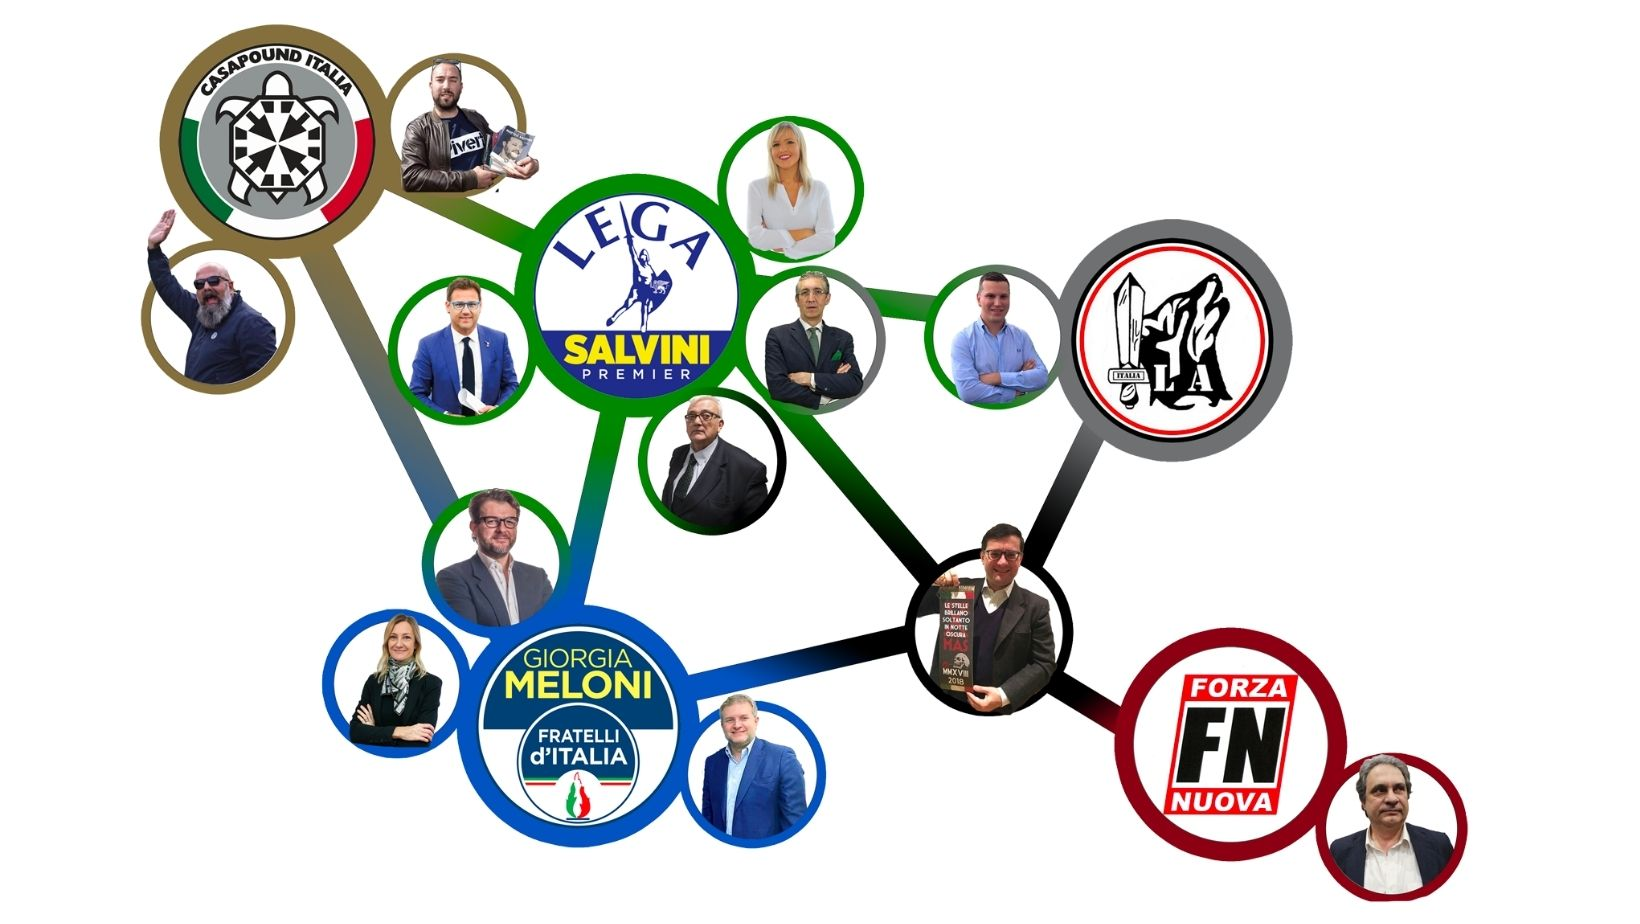
\includegraphics[width=0.5\textwidth,height=0.5\textheight]{https://www.cantiere.org/wp-content/uploads/2021/10/banner-NFVM.jpg}

\hypertarget{introduction}{%
\subsection{Introduction}\label{introduction}}

This first introductive work tries to highlight and recreate the
\emph{Itliaian ``Right'' network}. Especially in this period (after the
last victory of the Right-wing Coalition), in many case we heard talking
about some \emph{return to Fascism}. But it is really the case? We can
say that parties, like Lega or Fratelli d'Italia, are fascist parties? A
way that I figure out, trying to solve this \emph{dilemma}, is to
analyze the follower network of the Italian Far-right and Right-wings'
main Twitter profiles, and see if they share common followers.

\hypertarget{research-question-and-methodology}{%
\subsection{Research Question and
Methodology}\label{research-question-and-methodology}}

The main question is: is the Right-wing follower or community truly
``fascist''? If so, I think that they would be likely to follow also the
\emph{real} Italian Far-right parties and groups. So the main hypothesis
is: the ones who follows the Far-right communities and profiles would be
more likely to follow also the Right-wing communities, but not
viceversa, so the Right-wing followers will tend to follow only the
Right-wing communities and groups.

\hypertarget{twitter-lists}{%
\subsubsection{Twitter Lists}\label{twitter-lists}}

In order to do so, I create publics list on Twitter, which you can see
here:

\begin{itemize}
\tightlist
\item
  Far-right Culture:
  \url{https://twitter.com/i/lists/1600967243881451521}
\item
  Far-right Parties:
  \url{https://twitter.com/i/lists/1600600462612434969}
\item
  Right-wing Culture:
  \url{https://twitter.com/i/lists/1601188241394237442}
\item
  Right-wing Parties:
  \url{https://twitter.com/i/lists/1601142337874395136}
\end{itemize}

The \emph{Far-right Culture} contains newspaper, cultural associations,
communities and musical groups (like ``Il Primato Nazionale'' newspaper,
Presidio Milano or ``Hobbit'' musical group). The \emph{Far-right
Parties} contains the main parties and their youth movements (Forza
Nuova, Lotta Studentesca, Casapuond Italia, Blocco Studentesco, Lealtà
Azione, \ldots). The \emph{Right-wing Culture} contains newspaper,
cultural associations and public figure link to that political area (La
verità, Buttafuoco, Daniele Capezzone, Nicola Porro, \ldots). And
finally, the \emph{Right-wing Parties} contains the main parties and
political figures (Lega, Fratelli d'Italia, Giorgia Meloni, Matteo
Salvini, Ignazio La Russa, \ldots). One clarification has to be made,
due to the limited amount of ``real follower'' that the Far-right also
have in the political elections, not only on social media, I took in my
lists also all the local pages that I found of the far-right parties, in
order to gain more network to work with, also because, for example, only
Lega and Fratelli d'Italia togheter have a network of more than 200.000
follower, each. So to obtain some usable data I have done this
methodological assumption.

\hypertarget{work-flow}{%
\subsubsection{Work Flow}\label{work-flow}}

The main steps to do to get the data and analyse them:

\begin{itemize}
\tightlist
\item
  Get a Twitter Academic API
\item
  Make the list on Twitter
\item
  Gain the data from Twitter
\item
  Clear and export the data
\item
  First graphical analysis of the data
\end{itemize}

\hypertarget{data-and-results}{%
\subsection{Data and Results}\label{data-and-results}}

\hypertarget{raw-data}{%
\subsubsection{Raw Data}\label{raw-data}}

After obtaining the academic API from Twitter, I started to gain the
data using the \texttt{rtweet} package. First, using the
\texttt{lists\_members} function, I obtain all the IDs of the memeber of
the list and then I \texttt{tibble} them in a dataframes.

\begin{Shaded}
\begin{Highlighting}[]
\CommentTok{\# Example for the Far\_right Parties list:}
\FunctionTok{library}\NormalTok{(rtweet)}
\FunctionTok{auth\_as}\NormalTok{(}\StringTok{\textquotesingle{}XXX\textquotesingle{}}\NormalTok{)}
\NormalTok{far\_right\_parties }\OtherTok{=} \FunctionTok{lists\_members}\NormalTok{(}
  \AttributeTok{list\_id =} \StringTok{"1600600462612434969"}\NormalTok{,}
  \AttributeTok{slug =} \ConstantTok{NULL}\NormalTok{,}
  \AttributeTok{owner\_user =} \ConstantTok{NULL}\NormalTok{,}
  \AttributeTok{n =} \DecValTok{100}\NormalTok{,}
  \AttributeTok{cursor =} \StringTok{"{-}1"}\NormalTok{,}
  \AttributeTok{token =} \ConstantTok{NULL}\NormalTok{,}
  \AttributeTok{retryonratelimit =} \ConstantTok{NULL}\NormalTok{,}
  \AttributeTok{verbose =} \ConstantTok{TRUE}\NormalTok{,}
  \AttributeTok{parse =} \ConstantTok{TRUE}\NormalTok{,}
\NormalTok{)}


\NormalTok{name\_far\_right\_parties }\OtherTok{=} \FunctionTok{tibble}\NormalTok{(far\_right\_parties}\SpecialCharTok{$}\NormalTok{screen\_name)}
\end{Highlighting}
\end{Shaded}

To get all the followers of all the lists' users I firstly convert the
\texttt{screen\_names} in the tibble into a character vector to
automatize the process with a general function.

\begin{Shaded}
\begin{Highlighting}[]
\CommentTok{\# Tranform the values in a character vector:}
\NormalTok{list\_fr\_culture }\OtherTok{=} \FunctionTok{c}\NormalTok{(far\_right\_culture}\SpecialCharTok{$}\NormalTok{screen\_name)}
\end{Highlighting}
\end{Shaded}

\begin{Shaded}
\begin{Highlighting}[]
\NormalTok{list\_fr\_culture[}\DecValTok{7}\NormalTok{]}
\NormalTok{list\_fr\_culture[}\DecValTok{12}\NormalTok{] }

\NormalTok{[}\DecValTok{1}\NormalTok{] }\StringTok{"ddtmilano"}    
\NormalTok{[}\DecValTok{1}\NormalTok{] }\StringTok{"PresidioMilano"}

\CommentTok{\# Now it gave use all the Screen{-}Name of the profiles like single units, now we can automatize the get\_follower function with a general function}
\end{Highlighting}
\end{Shaded}

Now with a general function and \texttt{lapply} function we can download
all the followers of every single user in the lists.

\begin{Shaded}
\begin{Highlighting}[]
\CommentTok{\# Now we get the follower through rtweet, creating a general function to use:}

\NormalTok{getAllFollowers }\OtherTok{\textless{}{-}} \ControlFlowTok{function}\NormalTok{ (name) \{ }
\NormalTok{    user\_follower }\OtherTok{\textless{}{-}} \FunctionTok{get\_followers}\NormalTok{(name, }\AttributeTok{n=}\ConstantTok{Inf}\NormalTok{, }\AttributeTok{retryonratelimit =}\NormalTok{ T) }
  \CommentTok{\# we put inf to get all the followers and retryonratelimit = T to respect automatically the 15 minutes refresh time for the API}
    \FunctionTok{Sys.sleep}\NormalTok{(}\DecValTok{1}\NormalTok{)}\CommentTok{\# we put a system sleep of 1 sec to not overstimulate the server}
    \FunctionTok{return}\NormalTok{(user\_follower) \}}

\NormalTok{follower\_fr\_culture }\OtherTok{\textless{}{-}} \FunctionTok{lapply}\NormalTok{(}\AttributeTok{X =}\NormalTok{ list\_fr\_culture, }\AttributeTok{FUN =}\NormalTok{ getAllFollowers) }
\CommentTok{\# We use lapply to repeat the same function on all the profile in the list}
\end{Highlighting}
\end{Shaded}

After doing this for all the list we obtain four large list with all the
followers of the users and we have to transform them in dataframes using
the \texttt{purr} package.

\begin{Shaded}
\begin{Highlighting}[]
\FunctionTok{library}\NormalTok{(purrr)}

\CommentTok{\# By using map\_dfr from purrr package we can create a single tibble out of the tibbles contained in the large list automatically}
\NormalTok{df\_fr\_c }\OtherTok{\textless{}{-}} \FunctionTok{map\_dfr}\NormalTok{(follower\_fr\_culture, bind\_rows)}
\NormalTok{df\_fr\_p }\OtherTok{\textless{}{-}} \FunctionTok{map\_dfr}\NormalTok{(follower\_fr\_parties, bind\_rows)}
\NormalTok{df\_rw\_c }\OtherTok{\textless{}{-}} \FunctionTok{map\_dfr}\NormalTok{(follower\_rw\_culture, bind\_rows)}
\NormalTok{df\_rw\_p }\OtherTok{\textless{}{-}} \FunctionTok{map\_dfr}\NormalTok{(follower\_rw\_parties, bind\_rows)}
\end{Highlighting}
\end{Shaded}

Then I exported all the \emph{raw dataframes} in the \texttt{Data}
folder:

\begin{verbatim}
##                   from_id.to_id
## 1          2822819688;NeraRadio
## 2 1600189581986496521;NeraRadio
## 3 1597147409351692289;NeraRadio
## 4 1598698526212608000;NeraRadio
## 5 1598693665173639169;NeraRadio
## 6           423312009;NeraRadio
\end{verbatim}

So we have four raw dataframes:

\begin{itemize}
\tightlist
\item
  Far-right Culture: 48.897 followers
\item
  Far-right Parties: 124.852 followers
\item
  Right-wing Culture: 295.983 followers
\item
  Right-wing Parties: 317.547 followers
\end{itemize}

\hypertarget{data-cleaning}{%
\subsubsection{Data Cleaning}\label{data-cleaning}}

Now we ignore the duplicates, in every dataframe. The idea is to see who
are the followers of the four main groups (as they were single users
with all the followers) so: Far Right Cultures and Parties, Right-wing
Cultures and Parties.

\begin{Shaded}
\begin{Highlighting}[]
\FunctionTok{library}\NormalTok{(dplyr)}

\CommentTok{\# We specify also the coloumn from\_id (wich are the followers)}

\NormalTok{clean\_df\_fr\_c }\OtherTok{=}\NormalTok{ df\_fr\_c }\SpecialCharTok{\%\textgreater{}\%} \FunctionTok{distinct}\NormalTok{(from\_id, }\AttributeTok{.keep\_all =} \ConstantTok{TRUE}\NormalTok{)}

\NormalTok{clean\_df\_fr\_p }\OtherTok{=}\NormalTok{ df\_fr\_p }\SpecialCharTok{\%\textgreater{}\%} \FunctionTok{distinct}\NormalTok{(from\_id, }\AttributeTok{.keep\_all =} \ConstantTok{TRUE}\NormalTok{)}

\NormalTok{clean\_df\_rw\_c }\OtherTok{=}\NormalTok{ df\_rw\_c }\SpecialCharTok{\%\textgreater{}\%} \FunctionTok{distinct}\NormalTok{(from\_id, }\AttributeTok{.keep\_all =} \ConstantTok{TRUE}\NormalTok{)}

\NormalTok{clean\_df\_rw\_p }\OtherTok{=}\NormalTok{ df\_rw\_p }\SpecialCharTok{\%\textgreater{}\%} \FunctionTok{distinct}\NormalTok{(from\_id, }\AttributeTok{.keep\_all =} \ConstantTok{TRUE}\NormalTok{)}
\end{Highlighting}
\end{Shaded}

They are also exported as \emph{clean dataframes} in the
\texttt{Clean\ Followers\ DF} sub-folder (in the \texttt{Data} folder).

\begin{Shaded}
\begin{Highlighting}[]
\CommentTok{\# We want to create a general dataframe with all the followers, divided by the main group which they refer to:}
\CommentTok{\# First we see how many and which common followers the four main groups share}
\FunctionTok{library}\NormalTok{(tidyverse)}
\NormalTok{f\_fr\_c }\OtherTok{=}\NormalTok{ clean\_df\_fr\_c }\SpecialCharTok{\%\textgreater{}\%} 
  \FunctionTok{mutate}\NormalTok{(}\AttributeTok{to\_id =} \StringTok{"frc"}\NormalTok{) }\SpecialCharTok{\%\textgreater{}\%} 
  \FunctionTok{add\_column}\NormalTok{(}\AttributeTok{fllw1 =} \DecValTok{1}\NormalTok{) }\SpecialCharTok{\%\textgreater{}\%} 
  \FunctionTok{add\_column}\NormalTok{(}\AttributeTok{fllw2 =} \ConstantTok{NA}\NormalTok{) }\SpecialCharTok{\%\textgreater{}\%} 
  \FunctionTok{add\_column}\NormalTok{(}\AttributeTok{fllw3 =} \ConstantTok{NA}\NormalTok{) }\SpecialCharTok{\%\textgreater{}\%} 
  \FunctionTok{add\_column}\NormalTok{(}\AttributeTok{fllw4 =} \ConstantTok{NA}\NormalTok{)}

\NormalTok{f\_fr\_p }\OtherTok{=}\NormalTok{ clean\_df\_fr\_p }\SpecialCharTok{\%\textgreater{}\%} 
  \FunctionTok{mutate}\NormalTok{(}\AttributeTok{to\_id =} \StringTok{"frp"}\NormalTok{)}\SpecialCharTok{\%\textgreater{}\%} 
  \FunctionTok{add\_column}\NormalTok{(}\AttributeTok{fllw1 =} \ConstantTok{NA}\NormalTok{) }\SpecialCharTok{\%\textgreater{}\%} 
  \FunctionTok{add\_column}\NormalTok{(}\AttributeTok{fllw2 =} \DecValTok{1}\NormalTok{) }\SpecialCharTok{\%\textgreater{}\%} 
  \FunctionTok{add\_column}\NormalTok{(}\AttributeTok{fllw3 =} \ConstantTok{NA}\NormalTok{) }\SpecialCharTok{\%\textgreater{}\%} 
  \FunctionTok{add\_column}\NormalTok{(}\AttributeTok{fllw4 =} \ConstantTok{NA}\NormalTok{)}

\NormalTok{f\_rw\_c }\OtherTok{=}\NormalTok{ clean\_df\_rw\_c }\SpecialCharTok{\%\textgreater{}\%} 
  \FunctionTok{mutate}\NormalTok{(}\AttributeTok{to\_id =} \StringTok{"rwc"}\NormalTok{)}\SpecialCharTok{\%\textgreater{}\%} 
  \FunctionTok{add\_column}\NormalTok{(}\AttributeTok{fllw1 =} \ConstantTok{NA}\NormalTok{) }\SpecialCharTok{\%\textgreater{}\%} 
  \FunctionTok{add\_column}\NormalTok{(}\AttributeTok{fllw2 =} \ConstantTok{NA}\NormalTok{) }\SpecialCharTok{\%\textgreater{}\%} 
  \FunctionTok{add\_column}\NormalTok{(}\AttributeTok{fllw3 =} \DecValTok{1}\NormalTok{) }\SpecialCharTok{\%\textgreater{}\%} 
  \FunctionTok{add\_column}\NormalTok{(}\AttributeTok{fllw4 =} \ConstantTok{NA}\NormalTok{)}

\NormalTok{f\_rw\_p }\OtherTok{=}\NormalTok{ clean\_df\_rw\_p }\SpecialCharTok{\%\textgreater{}\%} 
  \FunctionTok{mutate}\NormalTok{(}\AttributeTok{to\_id =} \StringTok{"rwp"}\NormalTok{)}\SpecialCharTok{\%\textgreater{}\%} 
  \FunctionTok{add\_column}\NormalTok{(}\AttributeTok{fllw1=} \ConstantTok{NA}\NormalTok{) }\SpecialCharTok{\%\textgreater{}\%} 
  \FunctionTok{add\_column}\NormalTok{(}\AttributeTok{fllw2 =} \ConstantTok{NA}\NormalTok{) }\SpecialCharTok{\%\textgreater{}\%} 
  \FunctionTok{add\_column}\NormalTok{(}\AttributeTok{fllw3 =} \ConstantTok{NA}\NormalTok{) }\SpecialCharTok{\%\textgreater{}\%} 
  \FunctionTok{add\_column}\NormalTok{(}\AttributeTok{fllw4 =} \DecValTok{1}\NormalTok{)}

\NormalTok{tot\_followers }\OtherTok{=} \FunctionTok{rbind}\NormalTok{(f\_fr\_c, f\_fr\_p, f\_rw\_c, f\_rw\_p)}
\FunctionTok{colnames}\NormalTok{(tot\_followers) }\OtherTok{=} \FunctionTok{c}\NormalTok{(}\StringTok{"follower\_id"}\NormalTok{, }\StringTok{"grp"}\NormalTok{, }\StringTok{"fllw1"}\NormalTok{, }\StringTok{"fllw2"}\NormalTok{, }\StringTok{"fllw3"}\NormalTok{, }\StringTok{"fllw4"}\NormalTok{)}
\end{Highlighting}
\end{Shaded}

Now we can see how many followers each group has.
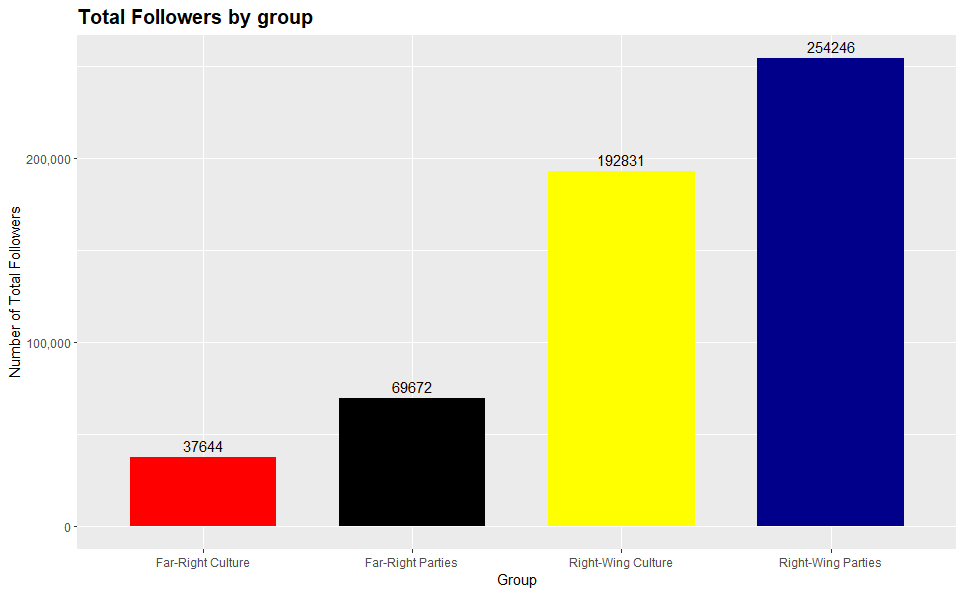
\includegraphics{https://github.com/DataAccess2020/Capstone_Taddei_Ita_Right/blob/main/Plots/Hist_Total_follower.png?raw=true}

As we can see, and as we wrote before, the Far-right area is very
limited compared to the Right-wing, also with the methodological
coercion that we settled. Now we want to see how many common and unique
followers there are, and what they follow:

\begin{Shaded}
\begin{Highlighting}[]
\NormalTok{id\_follow\_grp}\OtherTok{\textless{}{-}}\NormalTok{ tot\_followers }\SpecialCharTok{\%\textgreater{}\%}  \CommentTok{\# From the main dataframe}
  \FunctionTok{group\_by}\NormalTok{(follower\_id) }\SpecialCharTok{\%\textgreater{}\%}  \CommentTok{\# We keep our focus on the follower\_id, and group together the same row by the same follower\_id}
  \FunctionTok{summarise}\NormalTok{(}\AttributeTok{fllw1 =} \FunctionTok{sum}\NormalTok{(fllw1, }\AttributeTok{na.rm =}\NormalTok{ T),}
            \AttributeTok{fllw2 =} \FunctionTok{sum}\NormalTok{(fllw2, }\AttributeTok{na.rm =}\NormalTok{ T),}
            \AttributeTok{fllw3 =} \FunctionTok{sum}\NormalTok{(fllw3, }\AttributeTok{na.rm =}\NormalTok{ T),}
            \AttributeTok{fllw4 =} \FunctionTok{sum}\NormalTok{(fllw4, }\AttributeTok{na.rm =}\NormalTok{ T)) }\CommentTok{\# We sum all the properties of the single follower\_id (so if it follows other groups)}
\FunctionTok{colnames}\NormalTok{(id\_follow\_grp) }\OtherTok{=} \FunctionTok{c}\NormalTok{(}\StringTok{"follower\_id"}\NormalTok{, }\StringTok{"frc"}\NormalTok{, }\StringTok{"frp"}\NormalTok{, }\StringTok{"rwc"}\NormalTok{, }\StringTok{"rwp"}\NormalTok{) }\CommentTok{\# Rename columns to be more readable}
\end{Highlighting}
\end{Shaded}

So, now we have a very large dataframe with \textbf{447.810 Twitter
users} and what groups they follow.

\begin{verbatim}
##           follower_id frc frp rwc rwp
## 1 1000000732303675392   1   1   0   0
## 2          1000003220   0   1   0   0
## 3           100000643   0   0   0   1
## 4 1000009841224699904   1   0   0   0
## 5 1000014038850523136   1   1   0   1
## 6 1000014815589486592   1   1   0   0
\end{verbatim}

\hypertarget{data-analysis}{%
\subsubsection{Data Analysis}\label{data-analysis}}

With this first approach, I want to show how the groups' followers
network is connected between each other. In order to do so, I plot the
groups by subsetting them (with setted parameters,
\texttt{variable\ group\ ==\ 1}, so, in other terms, keeping
``costant'', group by group, only the ones who follow the
\emph{independent x group}) and then comparing with each other groups
using \texttt{ggplot2} package, and then with \texttt{gridExtra} package
and \texttt{plot\_grid} function I put the three plots (for each group).
Here it is a script example:

\begin{Shaded}
\begin{Highlighting}[]
\CommentTok{\# FAR RIGHT CULTURE}
\CommentTok{\# We subset the main dataframe to select only the one who follow the Far{-}Right Culture group, and see which other groups they follow}
\NormalTok{sub1 }\OtherTok{=} \FunctionTok{subset}\NormalTok{(id\_follow\_grp, frc }\SpecialCharTok{==} \DecValTok{1}\NormalTok{)}
\CommentTok{\# Far{-}Right Culture compared to Right{-}wing Culture}
\NormalTok{frc1 }\OtherTok{=} \FunctionTok{ggplot}\NormalTok{(sub1, }\FunctionTok{aes}\NormalTok{(}\FunctionTok{factor}\NormalTok{(frc), }\AttributeTok{fill =} \FunctionTok{factor}\NormalTok{(rwc))) }\SpecialCharTok{+}
  \FunctionTok{geom\_bar}\NormalTok{(}\AttributeTok{position=}\StringTok{"stack"}\NormalTok{)}\SpecialCharTok{+}
  \FunctionTok{geom\_text}\NormalTok{(}\FunctionTok{aes}\NormalTok{(}\AttributeTok{label =} \FunctionTok{paste0}\NormalTok{(}\FunctionTok{round}\NormalTok{(}\FunctionTok{after\_stat}\NormalTok{(count)}\SpecialCharTok{/}\FunctionTok{sum}\NormalTok{(count)}\SpecialCharTok{*}\DecValTok{100}\NormalTok{,}\DecValTok{1}\NormalTok{), }\StringTok{"\%"}\NormalTok{)), }\AttributeTok{stat =} \StringTok{"count"}\NormalTok{, }\AttributeTok{position =} \FunctionTok{position\_stack}\NormalTok{(}\AttributeTok{vjust =} \FloatTok{0.5}\NormalTok{), }\AttributeTok{colour =} \StringTok{"black"}\NormalTok{, }\AttributeTok{size =} \DecValTok{5}\NormalTok{) }\SpecialCharTok{+} \CommentTok{\# We put percentages to be more readable}
  \FunctionTok{xlab}\NormalTok{(}\StringTok{"Far{-}Right Culture Follower"}\NormalTok{) }\SpecialCharTok{+}
  \FunctionTok{ylab}\NormalTok{(}\StringTok{"Number of Total Followers"}\NormalTok{)}\SpecialCharTok{+} \CommentTok{\# We customize our plot axis}
  \FunctionTok{scale\_y\_continuous}\NormalTok{(}\AttributeTok{labels =}\NormalTok{ scales}\SpecialCharTok{::}\NormalTok{comma)}\SpecialCharTok{+}
  \FunctionTok{labs}\NormalTok{(}\AttributeTok{fill =} \StringTok{"Right{-}wing Culture"}\NormalTok{)}\SpecialCharTok{+} \CommentTok{\# We customize our plot legend}
  \FunctionTok{scale\_fill\_hue}\NormalTok{(}\AttributeTok{labels =} \FunctionTok{c}\NormalTok{(}\StringTok{\textquotesingle{}Not Follow\textquotesingle{}}\NormalTok{,}\StringTok{\textquotesingle{}Follow\textquotesingle{}}\NormalTok{))}\SpecialCharTok{+}
  \FunctionTok{coord\_flip}\NormalTok{() }\CommentTok{\# We put the plot in horizontal form}
\CommentTok{\# Far{-}Right Culture compared to RFar{-}Right Parties}
\NormalTok{frc2 }\OtherTok{=} \FunctionTok{ggplot}\NormalTok{(sub1, }\FunctionTok{aes}\NormalTok{(}\FunctionTok{factor}\NormalTok{(frc), }\AttributeTok{fill =} \FunctionTok{factor}\NormalTok{(frp))) }\SpecialCharTok{+}
  \FunctionTok{geom\_bar}\NormalTok{(}\AttributeTok{position=}\StringTok{"stack"}\NormalTok{)}\SpecialCharTok{+}
  \FunctionTok{geom\_text}\NormalTok{(}\FunctionTok{aes}\NormalTok{(}\AttributeTok{label =} \FunctionTok{paste0}\NormalTok{(}\FunctionTok{round}\NormalTok{(}\FunctionTok{after\_stat}\NormalTok{(count)}\SpecialCharTok{/}\FunctionTok{sum}\NormalTok{(count)}\SpecialCharTok{*}\DecValTok{100}\NormalTok{,}\DecValTok{1}\NormalTok{), }\StringTok{"\%"}\NormalTok{)), }\AttributeTok{stat =} \StringTok{"count"}\NormalTok{, }\AttributeTok{position =} \FunctionTok{position\_stack}\NormalTok{(}\AttributeTok{vjust =} \FloatTok{0.5}\NormalTok{), }\AttributeTok{colour =} \StringTok{"black"}\NormalTok{, }\AttributeTok{size =} \DecValTok{5}\NormalTok{) }\SpecialCharTok{+}
  \FunctionTok{xlab}\NormalTok{(}\StringTok{"Far{-}Right Culture Follower"}\NormalTok{) }\SpecialCharTok{+}
  \FunctionTok{ylab}\NormalTok{(}\StringTok{"Number of Total Followers"}\NormalTok{)}\SpecialCharTok{+}
  \FunctionTok{scale\_y\_continuous}\NormalTok{(}\AttributeTok{labels =}\NormalTok{ scales}\SpecialCharTok{::}\NormalTok{comma)}\SpecialCharTok{+}
  \FunctionTok{labs}\NormalTok{(}\AttributeTok{fill =} \StringTok{"Far{-}Right Parties"}\NormalTok{)}\SpecialCharTok{+}
  \FunctionTok{scale\_fill\_hue}\NormalTok{(}\AttributeTok{labels =} \FunctionTok{c}\NormalTok{(}\StringTok{\textquotesingle{}Not Follow\textquotesingle{}}\NormalTok{,}\StringTok{\textquotesingle{}Follow\textquotesingle{}}\NormalTok{))}\SpecialCharTok{+}
  \FunctionTok{coord\_flip}\NormalTok{()}
\CommentTok{\# Far{-}Right Culture compared to Right{-}wing Parties}
\NormalTok{frc3 }\OtherTok{=} \FunctionTok{ggplot}\NormalTok{(sub1, }\FunctionTok{aes}\NormalTok{(}\FunctionTok{factor}\NormalTok{(frc), }\AttributeTok{fill =} \FunctionTok{factor}\NormalTok{(rwp))) }\SpecialCharTok{+}
  \FunctionTok{geom\_bar}\NormalTok{(}\AttributeTok{position=}\StringTok{"stack"}\NormalTok{)}\SpecialCharTok{+}
  \FunctionTok{geom\_text}\NormalTok{(}\FunctionTok{aes}\NormalTok{(}\AttributeTok{label =} \FunctionTok{paste0}\NormalTok{(}\FunctionTok{round}\NormalTok{(}\FunctionTok{after\_stat}\NormalTok{(count)}\SpecialCharTok{/}\FunctionTok{sum}\NormalTok{(count)}\SpecialCharTok{*}\DecValTok{100}\NormalTok{,}\DecValTok{1}\NormalTok{), }\StringTok{"\%"}\NormalTok{)), }\AttributeTok{stat =} \StringTok{"count"}\NormalTok{, }\AttributeTok{position =} \FunctionTok{position\_stack}\NormalTok{(}\AttributeTok{vjust =} \FloatTok{0.5}\NormalTok{), }\AttributeTok{colour =} \StringTok{"black"}\NormalTok{, }\AttributeTok{size =} \DecValTok{5}\NormalTok{) }\SpecialCharTok{+}
  \FunctionTok{xlab}\NormalTok{(}\StringTok{"Far{-}Right Culture Follower"}\NormalTok{) }\SpecialCharTok{+}
  \FunctionTok{ylab}\NormalTok{(}\StringTok{"Number of Total Followers"}\NormalTok{)}\SpecialCharTok{+}
  \FunctionTok{scale\_y\_continuous}\NormalTok{(}\AttributeTok{labels =}\NormalTok{ scales}\SpecialCharTok{::}\NormalTok{comma)}\SpecialCharTok{+}
  \FunctionTok{labs}\NormalTok{(}\AttributeTok{fill =} \StringTok{"Right{-}wing Parties"}\NormalTok{)}\SpecialCharTok{+}
  \FunctionTok{scale\_fill\_hue}\NormalTok{(}\AttributeTok{labels =} \FunctionTok{c}\NormalTok{(}\StringTok{\textquotesingle{}Not Follow\textquotesingle{}}\NormalTok{,}\StringTok{\textquotesingle{}Follow\textquotesingle{}}\NormalTok{))}\SpecialCharTok{+}
  \FunctionTok{coord\_flip}\NormalTok{()}
\CommentTok{\# We merge all the three plots in one by using:}
\FunctionTok{install.packages}\NormalTok{(}\StringTok{"cowplot"}\NormalTok{)}
\FunctionTok{library}\NormalTok{(cowplot)}
\FunctionTok{plot\_grid}\NormalTok{(frc2, frc1, frc3, }\AttributeTok{nrow =} \DecValTok{3}\NormalTok{, }\AttributeTok{rel\_widths =} \FunctionTok{c}\NormalTok{(}\FloatTok{0.75}\NormalTok{,}\FloatTok{0.75}\NormalTok{, }\FloatTok{0.75}\NormalTok{))}\SpecialCharTok{+}
  \FunctionTok{ggtitle}\NormalTok{(}\StringTok{"Total Followers Far{-}Right Culture"}\NormalTok{)}\SpecialCharTok{+} \CommentTok{\# We put the main title}
  \FunctionTok{theme}\NormalTok{(}\AttributeTok{plot.title =} \FunctionTok{element\_text}\NormalTok{(}\AttributeTok{family =} \StringTok{"Helvetica"}\NormalTok{, }\AttributeTok{face =} \StringTok{"bold"}\NormalTok{, }\AttributeTok{size =}\NormalTok{ (}\DecValTok{15}\NormalTok{)))}
\end{Highlighting}
\end{Shaded}

After doing this for all the groups we obtain these polts:
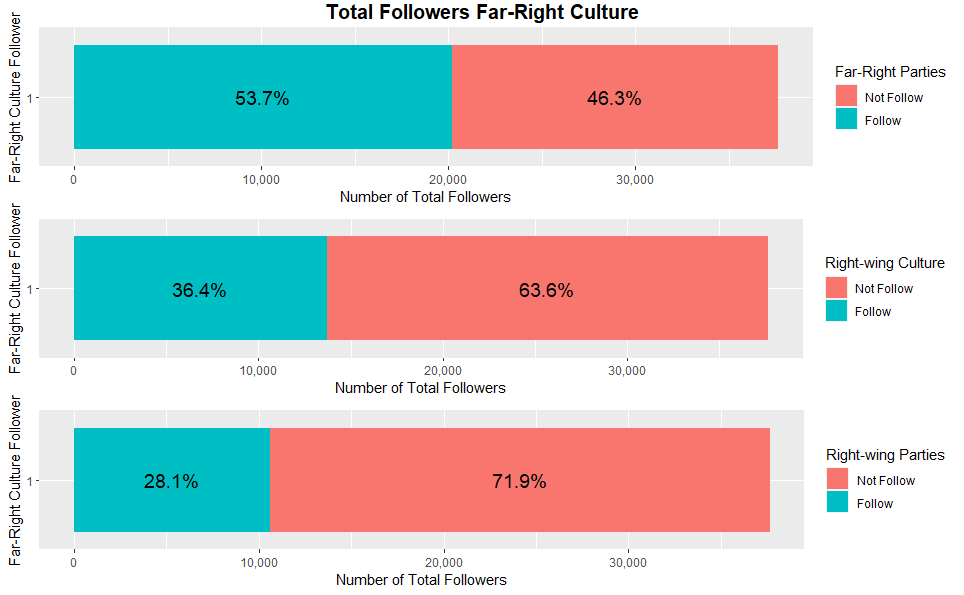
\includegraphics{https://github.com/DataAccess2020/Capstone_Taddei_Ita_Right/blob/main/Plots/FRC_confront_perc.png?raw=true}
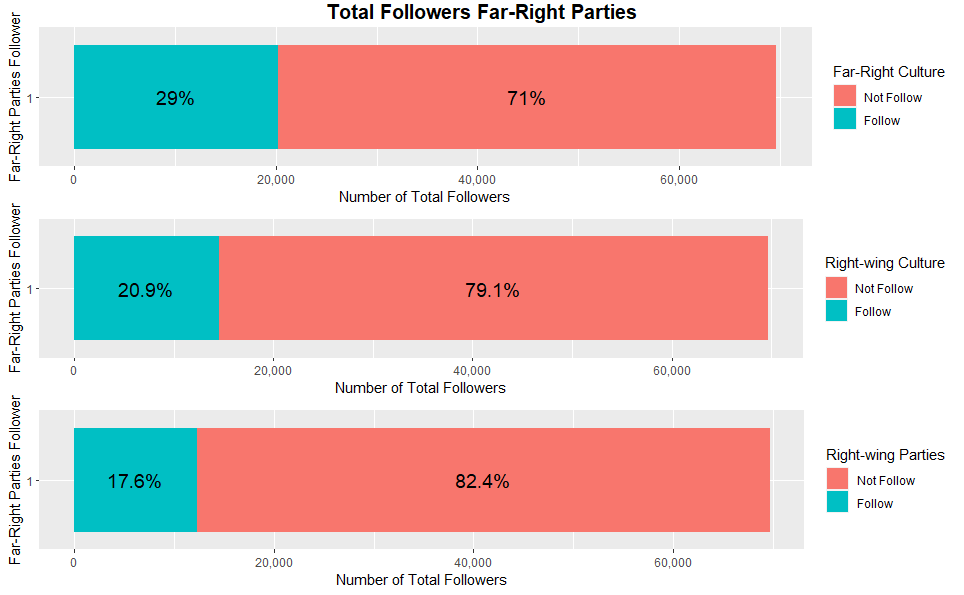
\includegraphics{https://github.com/DataAccess2020/Capstone_Taddei_Ita_Right/blob/main/Plots/FRP_confront_perc.png?raw=true}
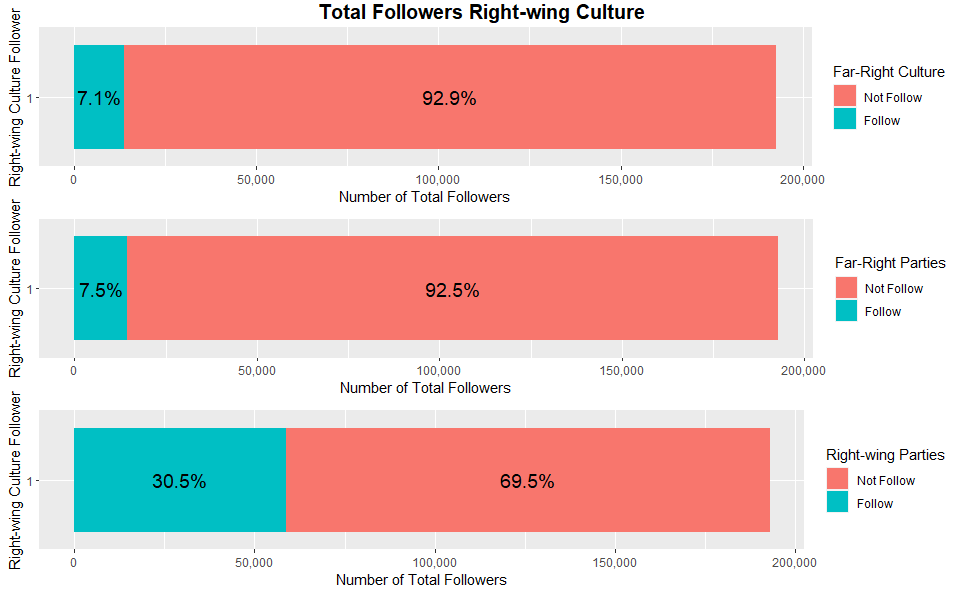
\includegraphics{https://github.com/DataAccess2020/Capstone_Taddei_Ita_Right/blob/main/Plots/RWC_confront_perc.png?raw=true}
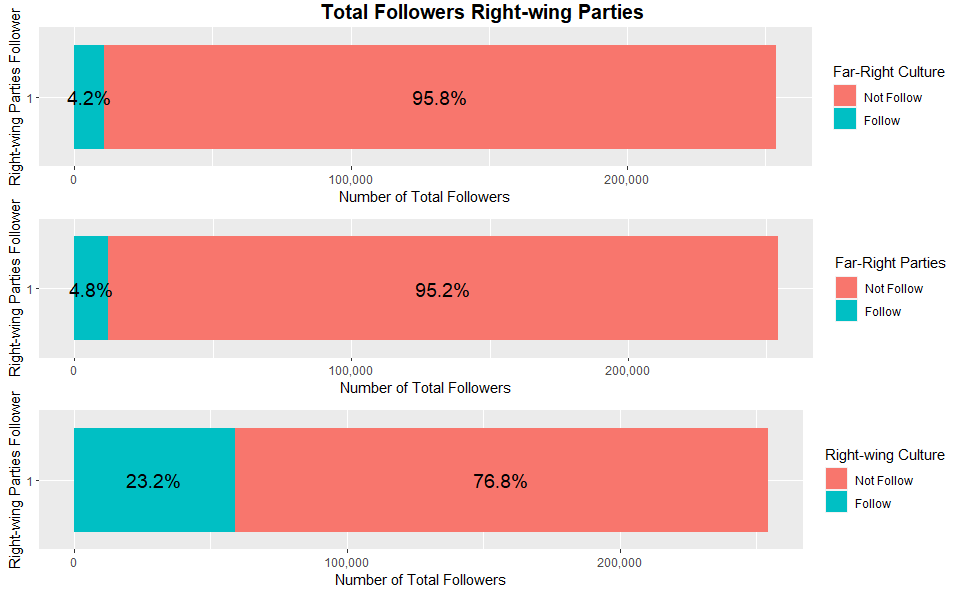
\includegraphics{https://github.com/DataAccess2020/Capstone_Taddei_Ita_Right/blob/main/Plots/RWP_confront_perc.png?raw=true}

\hypertarget{results} of the Far-right Culture group also follow the
  Far-right Parties group.
\item
  \textbf{29\%} of the Far-right Parties group also follow the Far-right
  Culture group.
\end{itemize}

In general we can say that, it seems that, on average, a third of the
ones who follow the Far-right Culture group also follow the other
political group. For the Right-wing group we can see that percentages of
common follower are very low, in regard of the Far-right group, with the
smallest percentages in the relation Right-wing Parites follower and all
the Far-right area. So it seems that Right-wing followers are not
interested in the Far-right movement or cultural area. But, on the other
hand, we can see a good connection within the Right-wing followers:
between the cultural and the political area.

\begin{itemize}
\tightlist
\item
  \textbf{30.5\%} of the Right-wing Culture group also follow the
  Right-wing Parties group.
\item
  \textbf{23.2\%} of the Right-wing Parties group also follow the
  Right-wing Culture group.
\end{itemize}

It's also interesting to see that, on average, one third of the
\emph{``Cultural followers''} also follow their Parties/political group,
but not viceversa. Interestingly, finally, the \emph{best} percentages
of common/shared followers come from the \textbf{Far-Right Culture
group}.

\hypertarget{final-conclusion}{%
\subsection{Final Conclusion}\label{final-conclusion}}

We see a primarily analysis on how the ``Italian Right'' it's connected
on Twitter, obviously it's a first approach and I really enjoy doing it.
I am sure that I have to extend the lists' members to gain the more
realistic results, in fact I have the suspect that I didn't reach all
the followers (I have this suspect especially for the Right-wing parties
list), so I will provide to correct and expand the lists. Initially I
was planning to use the \texttt{igraph} package to visualize also the
network, but I had some problems trying to figure out how to set the
\texttt{edges} and \texttt{vertex/nodes}, I think that maybe with the
next courses that we will take part, maybe I will gain the skills to do
this graphical visualization, for sure this project it's not finished,
and as soon as I will have the coding skill to do it, I will update this
project.

Finally, with this short research I would like to start a bigger project
(maybe the master thesis itself), trying to understand and analyse the
\emph{submerged} network of the ``Italian Right''. I think that our
Country has not close yet with its past. So analyzing, studying and
trying to understand why and how ``fascism'' (in different forms) still
survive nowdays and how the network spread (especially on social
network). I think that the best method to really understand our history
and move on is to have a scientific-analytic approach: my aim is to mix
the historic research (due to my previous degree in Political Science,
with a particular regard to history of political movement) with the
quantitative data analysis. Shouting or slogans will never permit a real
consciousness of what we are, where we came from and why so strong
political ideas still survive in our society.

\end{document}
